%%%%%%%%%%%%%% COPYRIGHT INFORMATION %%%%%%%%%%%%%%
% Template by
% Author: Sascha Frank 
% Nov. 2006
% University Freiburg 
% www.informatik.uni-freiburg.de/~frank/
% Distributed freely for non-commercial use

%%%%%%%%%%%%%%%%%%%%% PREAMBLE %%%%%%%%%%%%%%%%%%%%%
\documentclass{beamer}
\usepackage{beamerthemeshadow}
\usepackage{lmodern}
\usepackage{color}
\usepackage[]{url}

% include frame number on each frame
\setbeamertemplate{footline}{\quad \insertframenumber/\inserttotalframenumber}
\newcommand{\cmark}{\ding{51}} % check-mark
\newcommand{\xmark}{\ding{55}} % X-mark
\newcommand{\inv}{^{-1}}
\newcommand{\e}{\varepsilon}
\newcommand{\E}{\mathbb{E}}
\newcommand{\N}{\mathbb{N}}
\renewcommand{\P}{\mathbb{P}}
\newcommand{\R}{\mathbb{R}}
\newcommand{\Var}{\mathbb{V}}
\newcommand{\X}{\mathcal{X}}
\newcommand{\Y}{\mathcal{Y}}
\newcommand{\Z}{\mathcal{Z}}
\newcommand{\dist}{\operatorname{dist}}
\newcommand{\vi}{{\vec i}}
\newcommand{\sminus}{\backslash}

%%%%%%%%%%%%%%%%%%%%% DOCUMENT %%%%%%%%%%%%%%%%%%%%%
\begin{document}
\title{Low-Communication Distributed Optimization\\
       via E. Coli Swarm Foraging}
\author[Singh,Bar-Joseph]{Shashank Singh
\footnote{Carnegie Mellon University, Pittsburgh, PA, USA}
\and Saket Navlakha
\footnote{Salk Institute for Biological Studies, La Jolla, CA, USA}
\and Ziv Bar-Joseph$^1$
}
\institute{2nd Workshop on Biological Distributed Algorithms}
\date{October 12, 2014}

\section{Introduction}
\frame{\titlepage}

\subsection{Bacteria Swarm Foraging}
\frame{\frametitle{Differences from Insect Foraging}
\begin{center}
\begin{tabular}{l|l}
Insect Colonies & Bacteria Swarms   \\
\hline
\\
agents move food to colony \quad \quad \quad & \quad swarm moves to food \\\\
fixed pheromone trails & \quad diffusing protein signals \\\\
nurses, foragers, queen, etc. & \quad identical cells \\\\
complex navigation abilities & \quad no navigation ability
\end{tabular}
\end{center}
}

\frame{\frametitle{Bacteria Swarm Foraging}
\begin{columns}[T] % align columns
\begin{column}{.43\textwidth}
\begin{itemize}
\item Food source which diffuses with density $f : \R^2 \to \R$ throughout
solution
\item Obstacles
\item Bacteria swarms (typically $1$-$4$ swarms of $20$-$50$ agents each)
\end{itemize}
\end{column}%
\hfill%
\begin{column}{.8\textwidth}
\begin{figure}[h!]
  \centering
  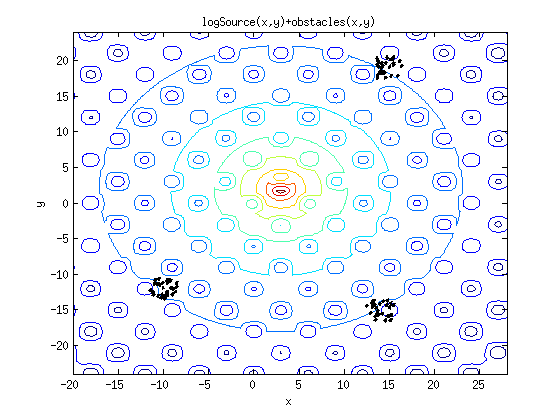
\includegraphics[width=1\linewidth]{setup}
\end{figure}
\end{column}
\end{columns}
}

\subsection{Computational Problem Statement}
\frame{\frametitle{Computational Problem}
Several nodes each want to maximize the same objective function:
\[\max_{x \in S \subseteq \R^d} f(x).\]
\begin{itemize}
\item can evaluate $f$, but don't know its form
\pause
\item $S$ and $f$ typically non-convex
\begin{itemize}
\item Can have small local maxima
\end{itemize}
\pause
\item Individual nodes computationally weak
\pause
\item Nodes can broadcast (small) messages to nearby nodes
\end{itemize}
}

\section{Old Model}
\subsection{Individual and Swarm Movement}
\frame{\frametitle{Individual Movement (Tumbling)}
Each iteration, each agent perturbs its direction based on previous change in
food density:
\vspace{-3mm}
\begin{columns}[T] % align columns
\begin{column}{.48\textwidth}
\[\delta = f(x_t,y_t) - f(x_{t - 1}, y_{t - 1})\]
\[\theta \to \theta + \e,
    \quad \mbox{ where } \quad \!\!\!\e \sim \mathcal{N}(0,\sigma^2),\]
\begin{figure}[h!]
  \centering
  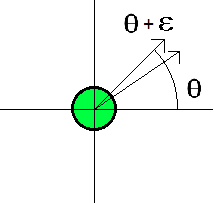
\includegraphics[width=0.4\linewidth]{theta_plus_epsilon}
\end{figure}
\end{column}%
\hfill%
\begin{column}{.6\textwidth}
\vspace{6mm}
\[\sigma \propto \max \left\{ 0, 1 - \delta \right\}.\]
\vspace{-7mm}
\begin{figure}[h!]
  \centering
  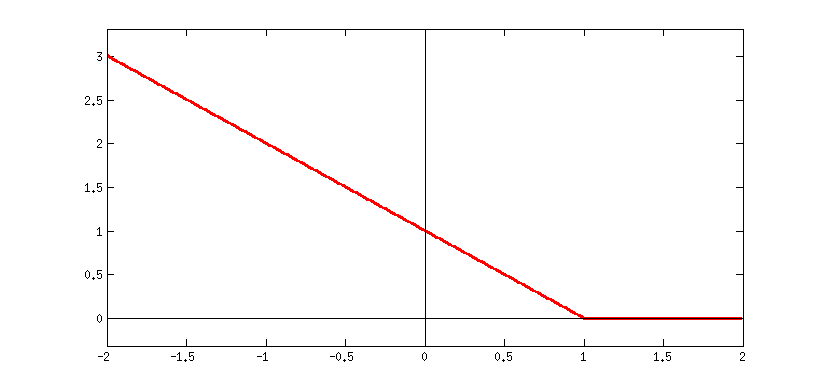
\includegraphics[width=\linewidth]{sigma_over_df}
\end{figure}
\end{column}
\end{columns}
}

\frame{\frametitle{Individual Movement (Tumbling)}
This works, but very inefficiently:
\begin{figure}[h!]
  \centering
  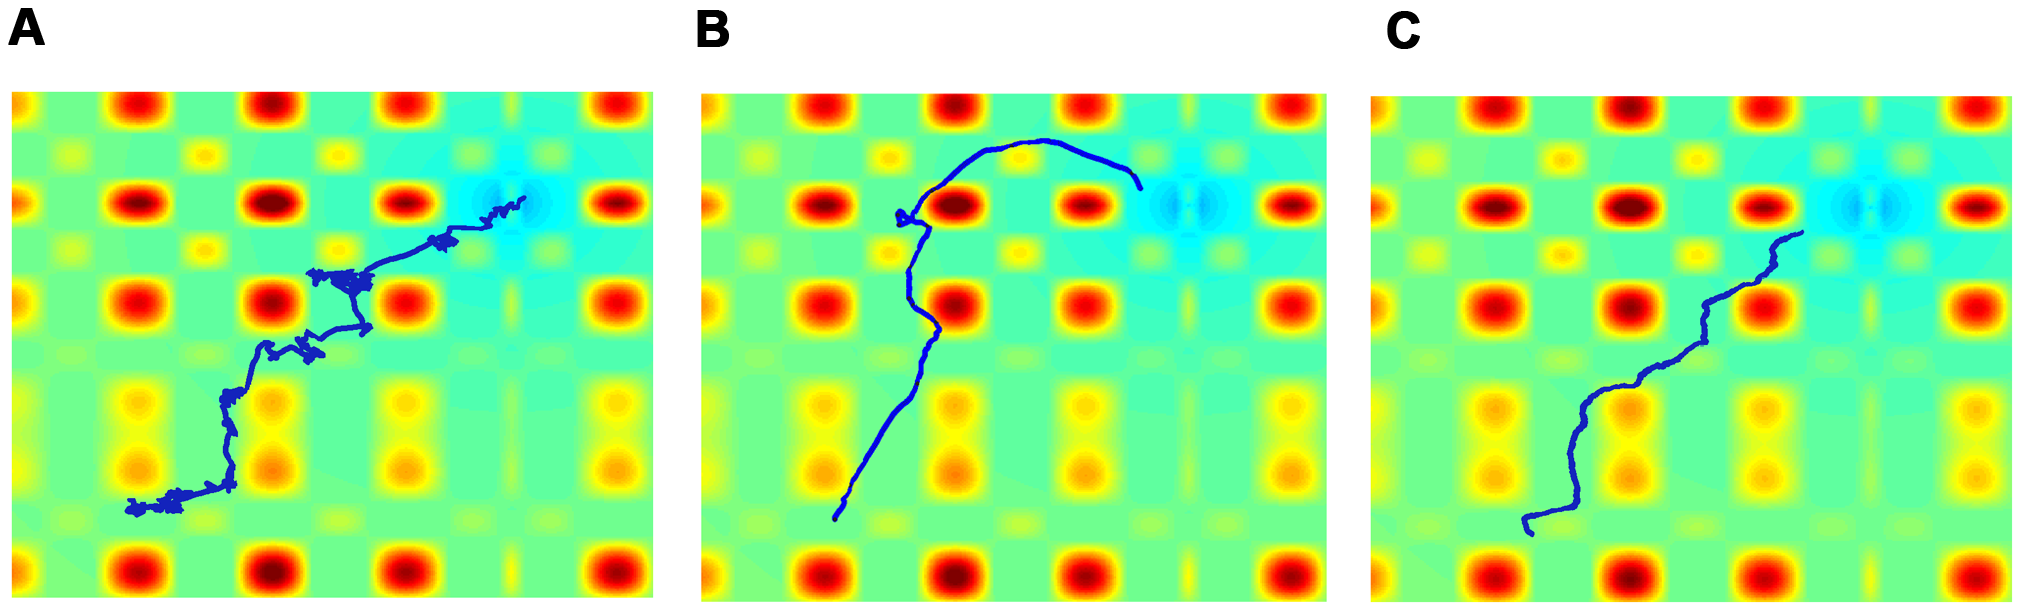
\includegraphics[trim=0mm 0mm 300mm 15mm, clip=true, width=0.6\linewidth]{single_agent}
\end{figure}
}

\frame{\frametitle{Basic Swarm Movement (Shklarsh et al., 2011)}
On each iteration, each agent combines its (perturbed) velocity with the
influence of the swarm
\[v_{i,t + 1}
    = w_v R_\e v_{i,t} + 
    \left\{
        \begin{array}{ll}
            w_r r_{i,t} & \mbox{ if any neighbors are too close } \\
            w_a a_{i,t} + w_\omega \omega_{i,t} & \mbox{ else}
        \end{array}
    \right.
\]
\begin{figure}[h!]
  \centering
  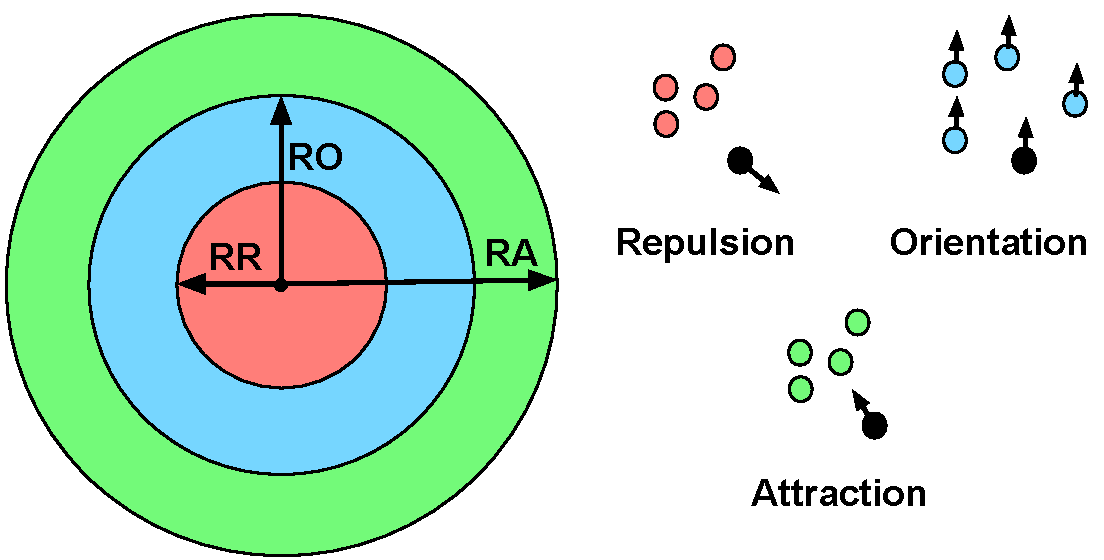
\includegraphics[width=0.8\linewidth]{comm}
\end{figure}
}

\subsection{Repulsion}
\frame{\frametitle{Basic Swarm Movement (Repulsion)}
Avoid collisions and spread out to cover area
\[r_{i,t}
    = \sum_{x_{j,t} \in B_{RR}(x_i)} \frac{x_{j,t} - x_{i,t}}{\|x_{j,t} - x_{i,t}\|}.\]
\begin{figure}[h!]
  \centering
  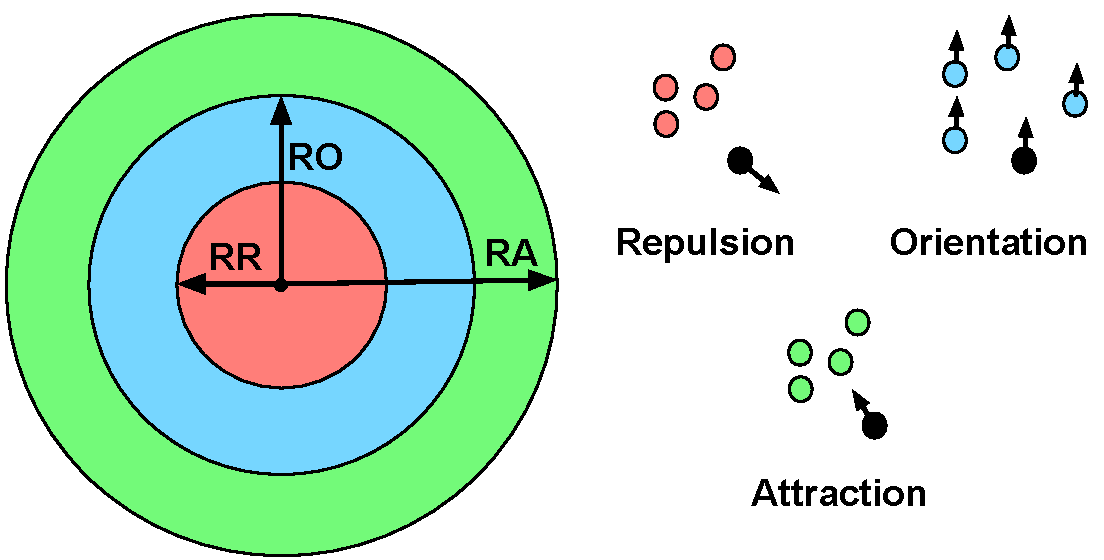
\includegraphics[width=0.8\linewidth]{comm}
\end{figure}
}

\subsection{Attraction}
\frame{\frametitle{Basic Swarm Movement (Attraction)}
Stay together as a group
\[a_{i,t}
    = \sum_{x_{j,t} \in B_{RA}(x_i)\sminus B_{RO(x_i)}}
                        \frac{x_{j,t} - x_{i,t}}{\|x_{j,t} - x_{i,t}\|}.\]
\begin{figure}[h!]
  \centering
  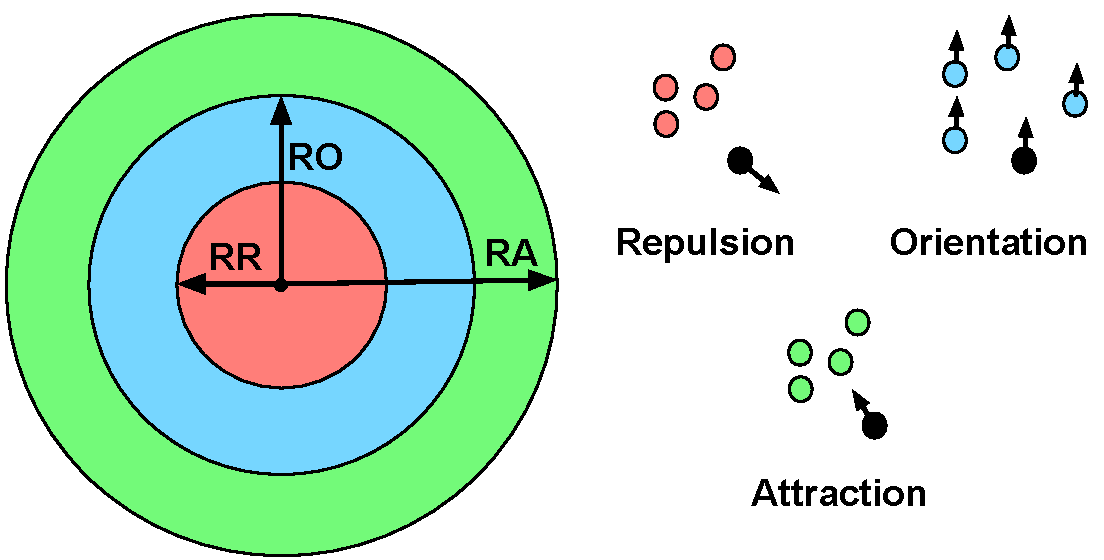
\includegraphics[width=0.55\linewidth]{comm}
\end{figure}
}

\subsection{Orientation}
\frame{\frametitle{Basic Swarm Movement (Orientation)}
Move similarly to your neighbors
\[\omega_{i,t} = \sum_{x_{j,t} \in B_{RO}(x_i)} \frac{v_{j,t}}{\|v_{j,t}\|}.\]
\begin{figure}[h!]
  \centering
  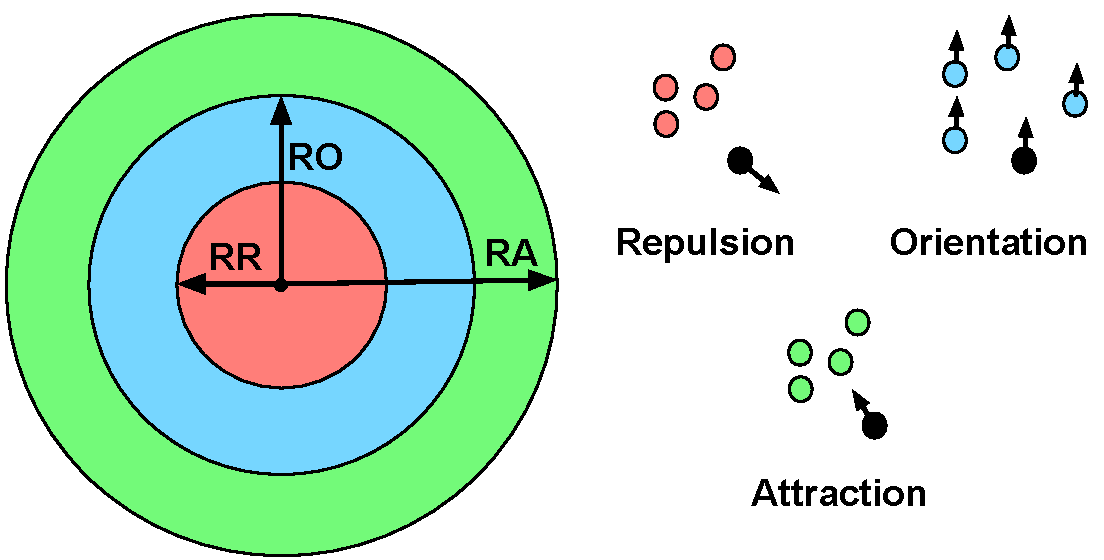
\includegraphics[width=0.55\linewidth]{comm}
\end{figure}
\pause
\begin{itemize}
\item Accelerates swarm when the correct direction is clear
\pause
\item Helps ``smooth'' interactions by preventing collisions.
\end{itemize}
}

\frame{\frametitle{Basic Swarm Movement (Shklarsh et al.)}
Again,
\[v_{i,t + 1}
    = w_v R_\e v_{i,t} + 
    \left\{
        \begin{array}{ll}
            w_r r_{i,t} & \mbox{ if any neighbors are too close } \\
            w_a a_{i,t} + w_\omega \omega_{i,t} & \mbox{ else}
        \end{array}
    \right.
\]
\begin{figure}[h!]
  \centering
  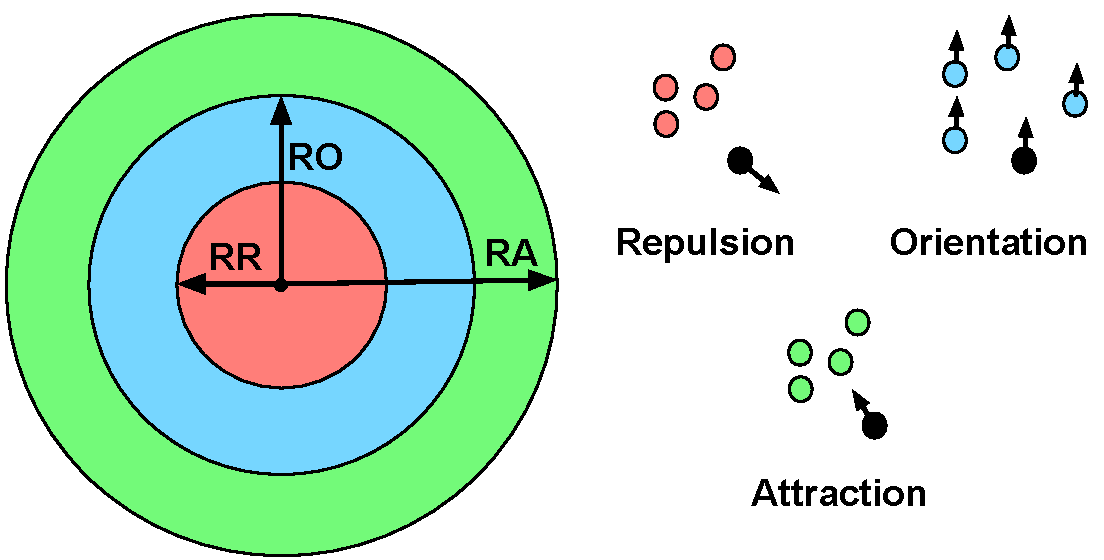
\includegraphics[width=0.8\linewidth]{comm}
\end{figure}
}

\section{New Model}
\subsection{Issues and Fixes}
\frame{\frametitle{Issues}
The Basic Swarm Movement model makes unrealistic assumptions about how bacteria
communicate orientation and attraction.
\pause
\[a_{i,t}
    = \sum_{x_{j,t} \in B_{RA}(x_i)\sminus B_{RO(x_i)}}
                        \frac{x_{j,t} - x_{i,t}}{\|x_{j,t} - x_{i,t}\|}
    \quad \mbox{ and } \quad
    \omega_{i,t}
    = \sum_{x_{j,t} \in B_{RO}(x_i)} \frac{v_{j,t}}{\|v_{j,t}\|}
\]
\begin{itemize}
\item Messages can be continuous (e.g., floats)
\pause
\begin{itemize}
\item Real bacteria send protein signals of only a few bits
\end{itemize}
\pause
\item Receiver's measurements can be arbitrarily large
\pause
\begin{itemize}
\item Real bacteria distinguish only a few levels
\end{itemize}
\end{itemize}
}

\frame{\frametitle{Discretization and Thresholding}
\begin{itemize}
\item Introduce a thresholding discretization function:
\begin{itemize}
\item For $T > 0$, $L \in \N$, $\|D_{L,T}(x)\| = \min\{T,\lfloor L\|x\|\rfloor/L\}$.
\item Approximate vectors by cardinal vectors to discretize direction
\end{itemize}
\end{itemize}
\vspace{-3mm}
\begin{columns}[T] % align columns
\begin{column}{.48\textwidth}
\begin{figure}[h!]
  \centering
  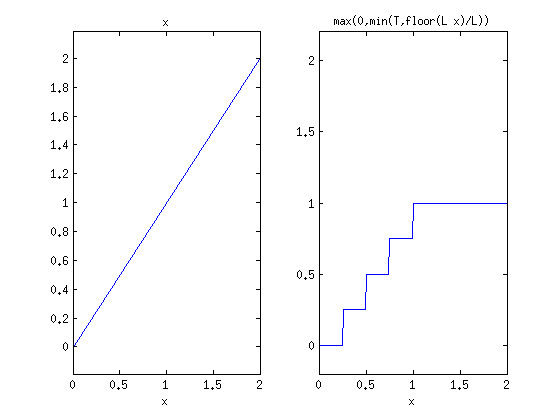
\includegraphics[trim=0mm 0mm 0mm 8mm, clip=true, width=1.3\linewidth]{discretization}
\end{figure}
\end{column}%
\hfill%
\begin{column}{.4\textwidth}
\begin{figure}[h!]
  \centering
  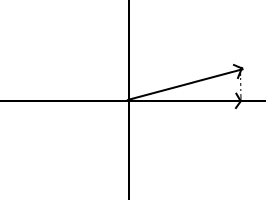
\includegraphics[width=1\linewidth]{snap_to_cardinal}
\end{figure}
\end{column}
\end{columns}
}

\frame{\frametitle{Issues (Cont.)}
The Basic Swarm Movement model makes unrealistic assumptions about how bacteria
communicate orientation and attraction (repulsion is ok).
\begin{figure}[h!]
  \centering
  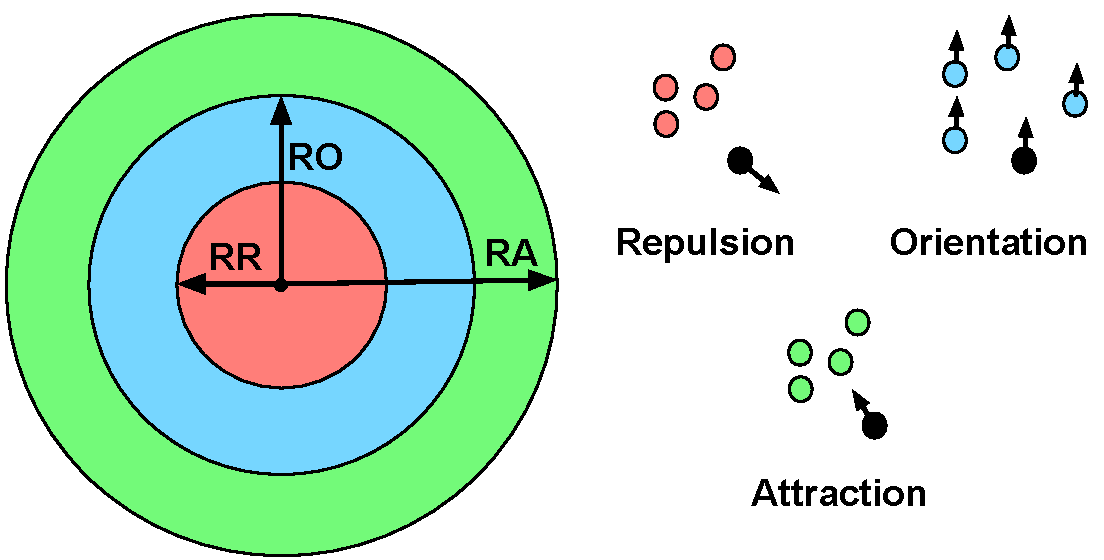
\includegraphics[width=0.6\linewidth]{comm}
\end{figure}
\vspace{-2mm}
\begin{itemize}
\item Agents can identify message senders (dedicated channels)
\begin{itemize}
\item Requires $\log (n)$ extra bits per message
\item Swarm can be dynamic
\item Real bacteria broadcast to their neighbors
\end{itemize}
\pause
\item Ability to communicate is unaffected by distance
\end{itemize}
}

\frame{\frametitle{Distance Weighting}
\begin{itemize}
\item Broadcast messages, but weight communication by distance
\begin{itemize}
\item Messages decay exponentially with distance:
$w_a(x) = \exp(-c_a x)$, \quad $w_\omega(x) = \exp(-c_\omega x)$
\quad ($c_\omega > c_a$)
\end{itemize}
\end{itemize}
\begin{columns}[T] % align columns
\begin{column}{.48\textwidth}
\begin{figure}[h!]
  \centering
  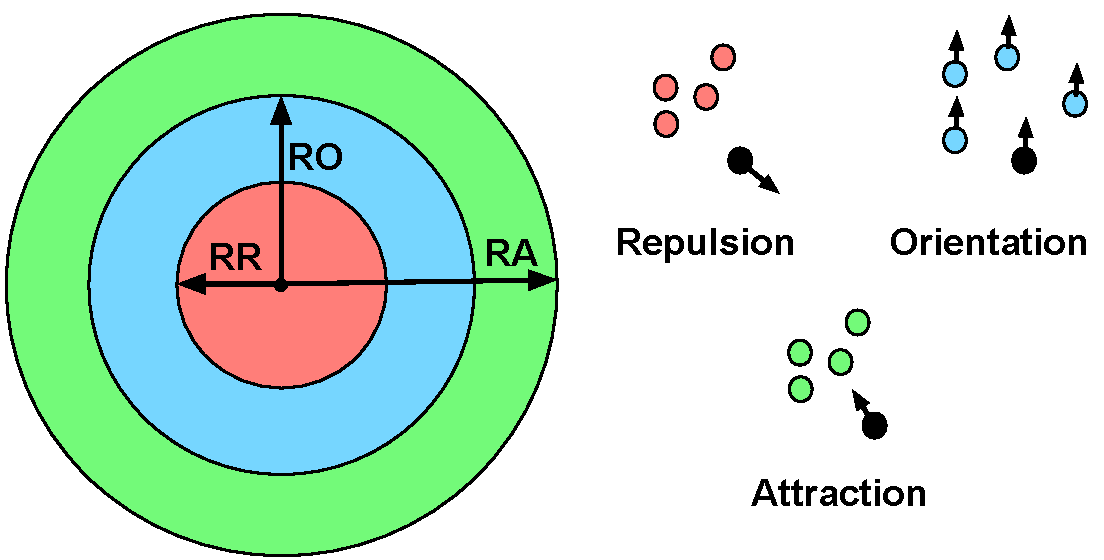
\includegraphics[trim=0mm 0mm 90mm 0mm, clip=true, width=\linewidth]{comm}
\end{figure}
\end{column}%
\hfill%
\begin{column}{.6\textwidth}
\begin{figure}[h!]
  \centering
  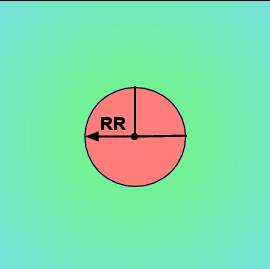
\includegraphics[trim=0mm 0mm 0mm 5mm, clip=true, width=0.85\linewidth]{comm2}
\end{figure}
\end{column}
\end{columns}
}

\subsection{Efficient Communication Model}
\frame{\frametitle{Efficient Communication Model}
\begin{itemize}
\item Discretize after weighting:
\end{itemize}
\[a_{i,t}
    = \sum_{j = 1}^n D_{L,T} \left(
        w_a(\|x_j - x_i\|)\frac{(x_j - x_i)}{\|x_j - x_i\|}
    \right)
\]
\[\omega_{i,t}
    = \sum_{j = 1}^n D_{L,T} \left(
        w_a(\|v_{j,t}\|)\frac{v_j}{\|v_j\|}
    \right)
\]
Recall
\[v_{i,t + 1}
    = w_v v_{i,t} + 
    \left\{
        \begin{array}{ll}
            w_r r_{i,t} & \mbox{ if any neighbors are too close } \\
            w_a a_{i,t} + w_\omega \omega_{i,t} & \mbox{ else}
        \end{array}
    \right.
\]
}

\subsection{Experimental Results}
\frame{\frametitle{Experimental Results}
\begin{figure}[h!]
  \centering
  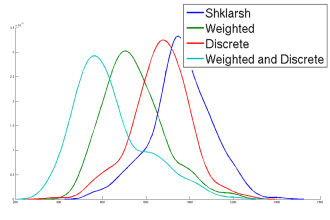
\includegraphics[width=0.8\linewidth]{shklarsh_vs_dwexp}\\
  \vspace{-3mm}
  {\scriptsize Path Length}
\end{figure}
}

\section{Extensions}
\subsection{Adaptive Listening}
\frame{\frametitle{Adaptive Listening}
Help if you're making progress, get help if you're stuck
\begin{itemize}
\item weight current velocity based on performance
\end{itemize}
Modified model:
\[v_t = w(\delta) \cdot v_{t - 1} + (1 - w(\delta))u,\]
where $w$ is increases with $\delta = f(x_t,y_t) - f(x_{t - 1},y_{t - 1})$.
}

% \subsection{Multiple Swarms}
% \frame{\frametitle{Multiple Swarms}
% \url{http://www.contrib.andrew.cmu.edu/~sss1/videos/}
% }
% 
\subsection{Silent Agents}
\frame{\frametitle{Silent Agents}
\begin{itemize}
\item broadcasting messages takes energy
\item many messages are redundant
\item under scarce resources, may not want to help competition
\end{itemize}
\pause
Modified model: For some $p_s \in [0,1]$, each agent is silent with probability
$p_s$.
}

\frame{\frametitle{Experimental Results: Silent Agents}
\begin{columns}[T] % align columns
\begin{column}{.5\textwidth}
\begin{figure}[h!]
  \centering
  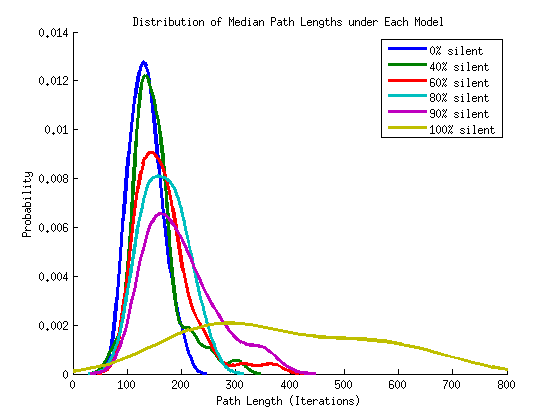
\includegraphics[width=1.2\linewidth]{dwexp_silents30}
\end{figure}
\end{column}%
\hfill%
\begin{column}{.6\textwidth}
\begin{figure}[h!]
  \centering
  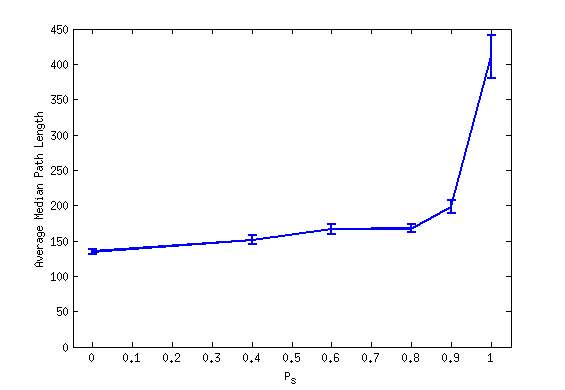
\includegraphics[width=1.1\linewidth]{dwexp_silents30_means}
\end{figure}
\end{column}
\end{columns}
\begin{center}
Very few agents actually need to communicate!
\end{center}
}

\frame{\frametitle{Summary}
\begin{itemize}
\item Primitive bacteria solve computationally challenging problems
collectively
\item Swarm communication is helpful even under highly restricted communication
\begin{itemize}
\item Agents need only broadcast a few bits
\item Signals only need need to travel short distances
\item Only some agents need to communicate
\end{itemize}
\end{itemize}
}

\frame{\frametitle{Future Work}
\begin{itemize}
\item Consider competition (finite food sources)
\item Multiple food sources/mixed objectives
\begin{itemize}
\item Agents can have different preferences
\end{itemize}
\item Compare to biological model
\begin{itemize}
\item Can identify genes responsible for communication?
\item How is orientation really communicated?
\end{itemize}
\item Theory
\begin{itemize}
\item Convergence rates
\item Lower bounds
\end{itemize}
\end{itemize}
}

\frame{\frametitle{\null}
\begin{center}
{\LARGE Thanks!}\\
\vspace{15mm}
Simulation code is available on GitHub.\\
\url{https://github.com/sss1/bact-sim/}
\end{center}
}
\end{document}  
